
%%%%%%%%%%%%%%%%%%%%%%%%%%%%%%%%%%%%%%%%%%%%%%%%%%%%%%%%%%%%%%%%%%%%%%%%
%Para las ecuaciones siempre es Ec.(n).
%Para las figuras siempre es Fig.n, incluso en el caption de la figura. Tambien las Tablas
%Para las referencias es [n]
%%%%%%%%%%%%%%%%%%%%%%%%%%%%%%%%%%%%%%%%%%%%%%%%%%%%%%%%%%%%%%%%%%%%%%%%

\documentclass[
reprint,
%notitlepage,
%superscriptaddress,
%groupedaddress,
%unsortedaddress,
%runinaddress,
%frontmatterverbose, 
%preprint,
%showpacs,preprintnumbers,
%nofootinbib,
%nobibnotes,
%bibnotes,
%11 pt,
amsmath,
amssymb,
aps,
pra,
%prb,
%rmp,
%tightenlines %esto hizo el milagro de sacar los espacios en blancos estocásticos (?)
 %prstab,
%prstper,
%floatfix,\textbf{}
]{revtex4-1} %Instalar primero para usarlo. Paquete malo.

%\documentclass[onecolumn, aps, amsmath,amssymb ]{article}
\usepackage{lipsum}  
\usepackage{graphicx}% Include figure files
\usepackage{subfig}
\usepackage{braket}
\usepackage{comment} %comment large chunks of text
\usepackage{dcolumn}% Align table columns on decimal point
\usepackage{bm}% bold math
%\usepackage{hyperref}% add hypertext capabilities
\usepackage[mathlines]{lineno}% Enable numbering of text and display math
%\linenumbers\relax % Commence numbering lines
\usepackage{mathtools} %% Para el supraíndice

\usepackage[nice]{nicefrac}

%%%%%%%El Señor Español%%%%%%%%%%%%%%%%%%%%%%%%%%%
\usepackage[utf8]{inputenc} %acento
\usepackage[
spanish, %El lenguaje.
es-tabla, %La tabla y no cuadro.
activeacute, %El acento.
es-nodecimaldot %Punto y no coma con separador de números
]{babel}
\usepackage{microtype} %para hacerlo más bonito :33 como vos (?) 
%%%%%%%%%%%%%%%%%%%%%%%%%%%%%%%%%%%%%%%%%%%%%%%%%%%
%%%%%%%%% Para que las imágenes se queden dónde las quiero (?
\usepackage{float}
%%%%%%%%%%

%%%%%%%%Cambia a Fig de Figure%%%%%%%%%%
\makeatletter
\renewcommand{\fnum@figure}{Fig. \thefigure} 
\makeatother
%%%%%%%%%%%%%%%%%%%%%%%%%%%%%%%%%%%%%%%%
\raggedbottom


\begin{document}
%%%%%%%%%%%%%%%%%%%%%%%%%%%%%%%%%%Título%%%%%%%%%%%%%%%%%%%%%%%%%%%%%%%%%%%%%%
%%%%%%%%%%%%%%%%%%%%%%%%%%%%%%%%%%%%%%%%%%%%%%%%%%%%%%%%%%%%%%%%%%%%%%%%%%%%%%

\title{Práctica 6: Memorias Asociativas}
\author{Evelyn~G.~Coronel}

\affiliation{
Redes Neuronales - Instituto Balseiro\\}

\date[]{\lowercase{\today}} %%lw para lw, [] sin date


\maketitle
%%%%%%%%%%%%%%%%%%%%%%%%%%%%%%%%%%%%%%%%%%%%%%%%%%%%%%%%%%%%%%%%%%%%%%%%%%%%%%%%%%%
% Podemos usar cualquiera de los dos comandos: \input o \include para incluir el texto
%\input{./Capitulo1/cap1.tex}

\subsection*{Cuestiones generales del modelo  de Hopfield}

El modelo de Hopfield contempla la idea de solucionar de la manera más simple el problema de memorizar patrones. Este problemas consiste en memorizar un conjunto de patrones $\xi^\mu _i$, de tal manera que si se presenta un patrón $\zeta^\mu_i$, la red responde con una salida que más se parece a la entrada dada. (PONER ref)

La red almacena $p$ patrones, que se indexan con $\mu=1, \dots, p$, mientras que las unidad dentro de la red se indexan mediante $i=1, \dots, N$. La convención que se toma en este trabajo es que cada patrón $\xi^\mu _i$ puede valer $+1$ o $-1$.
\subsubsection*{Salida de la red  para varios patrones}

Se define la matriz de conexiones $w_ij$, que tiene un parecido con una matriz de pesos, según la Ec. \ref{pesos}.
\begin{equation}
	w_{ij} = \frac{1}{N} \sum _{\mu=1} ^{p}\xi_i^\mu \xi_j^\mu 
	\label{pesos}
\end{equation}
donde el índice $i, j= 1, \dots , N$ recorre las unidades de la red y el índice $\nu= 1, \dots, p$ recorre el conjunto de patrones.

Dada una entrada $\zeta ^\mu_i$, definamos el parámetro $h^\nu_i $ como $h^\nu_i = \sum_j w_{ij} \xi_j ^\nu$. Para la validación de las redes de esta práctica, se utilizaron los mismos patrones almacenados con entrada de la red. 

\subsubsection*{Sobre la actualización}

Se toma una regla de actualización asincrónica, esta implica que:

\begin{itemize}
	\item En cada época, se selecciona una unidad i a ser actualizada aplicando la regla de la Ec.\,(\ref{eq:hop_gen})
	\item Cada unidad elige independientemente actualizarse o no, con una probabilidad en cada época. 
\end{itemize}

Para el modelo de Hopfield sin ruido, la probabilidad es constante en cada actualización es igual a $0.5$, es decir, se actualiza a cada paso con $+1$ o con $-1$. En cambio, para el modelo de Hopfield con ruido, la probabilidad de cambio está dada por una función que depende de la salida $h_i$ y de otro parámetro que simula un ruido térmico.


\section*{Ejercicio I: El modelo de Hopfield sin ruido}

Definamos el parámetro de carga $\alpha  = \nicefrac{p}{N}$, que es el números de patrones a almacenar como fracción 

\begin{equation}
	s(t+1)=  \begin{cases} 
   +1 & \text{Probabilidad }0.5 \\
   -1 & \text{Probabilidad }0.5 
\end{cases}
\end{equation}

La condición de estabilidad se generaliza a

\begin{equation}
	sgn(h^\nu _i ) = \xi_i^\nu \quad \forall \,i
\end{equation}


\begin{equation}
	S_i := sgn(\sum_j w_{ij} S_j - \theta_i)
\end{equation}
donde $sgn(x)$ es la función signo.

Para el resto del trabajo, el valor de $\theta_i=0$.

\begin{equation}
	S_i := sgn(\sum_j w_{ij} S_j)
	\label{eq:hop_gen}
\end{equation}



\subsection{Resultados}


\begin{figure}[H]
	\centering
	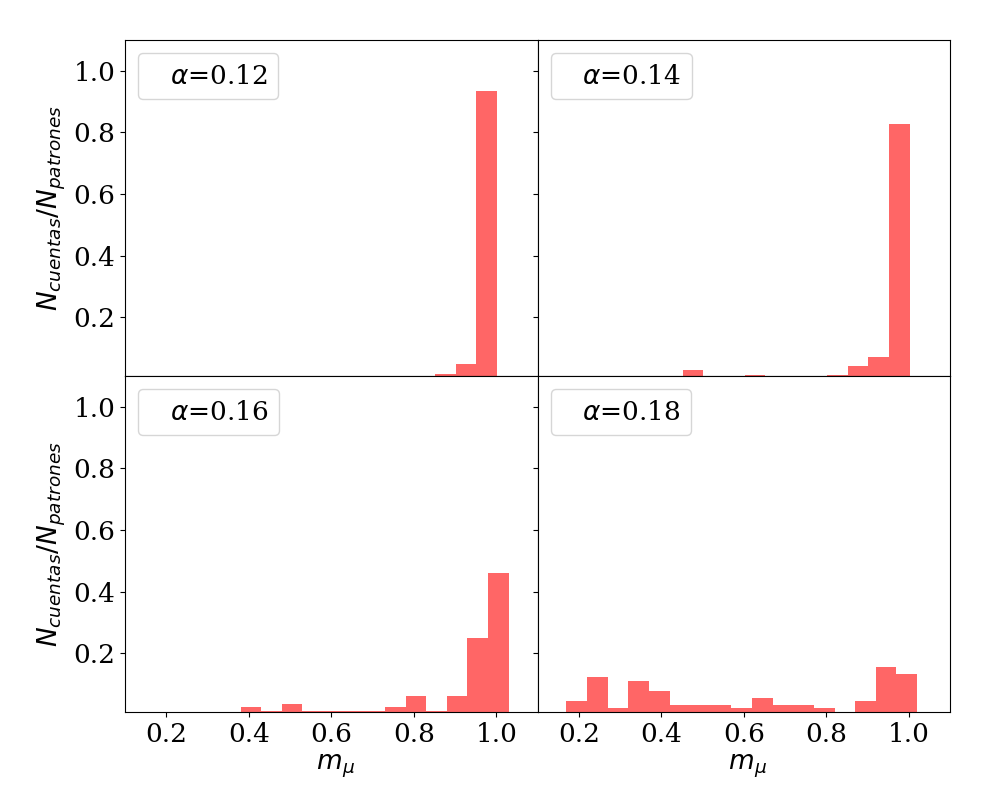
\includegraphics[width=0.5\textwidth]{../Graficos/500.png}
	\caption{Para $N=500$}
	\label{fig:500}
\end{figure}



\begin{figure}[H]
	\centering
	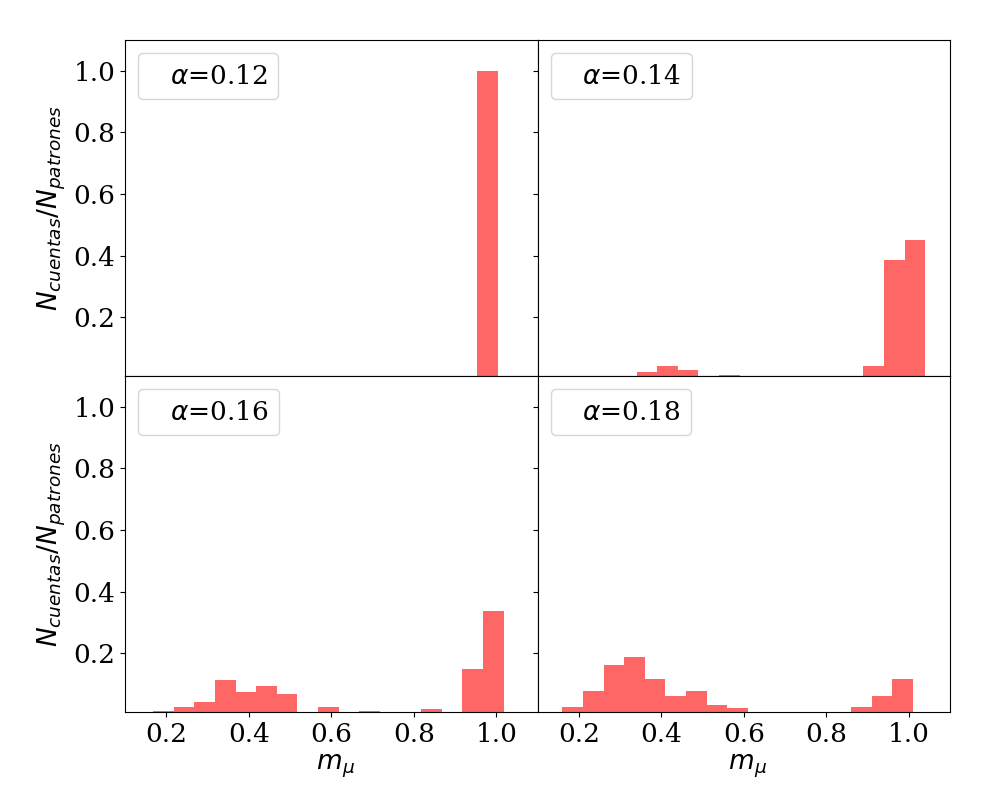
\includegraphics[width=0.5\textwidth]{../Graficos/1000.png}
	\caption{Para $N=1000$}
	\label{fig:1000}
\end{figure}


\begin{figure}[H]
	\centering
	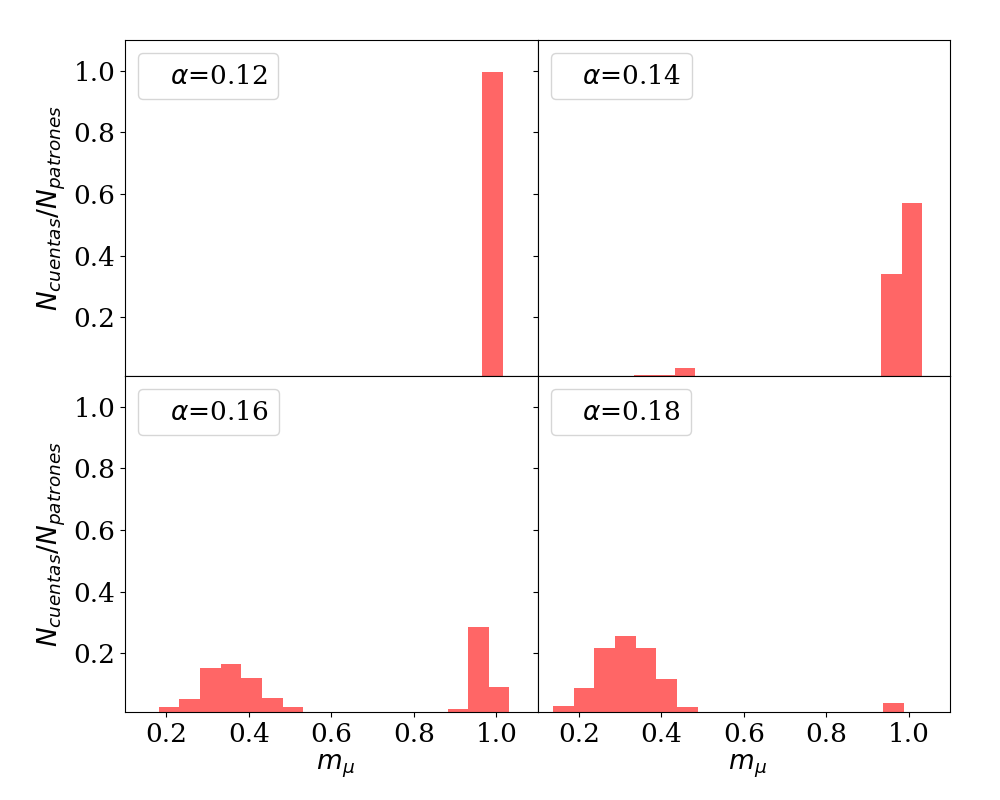
\includegraphics[width=0.5\textwidth]{../Graficos/2000.png}
	\caption{Para $N=2000$}
	\label{fig:2000}
\end{figure}



\begin{figure}[H]
	\centering
	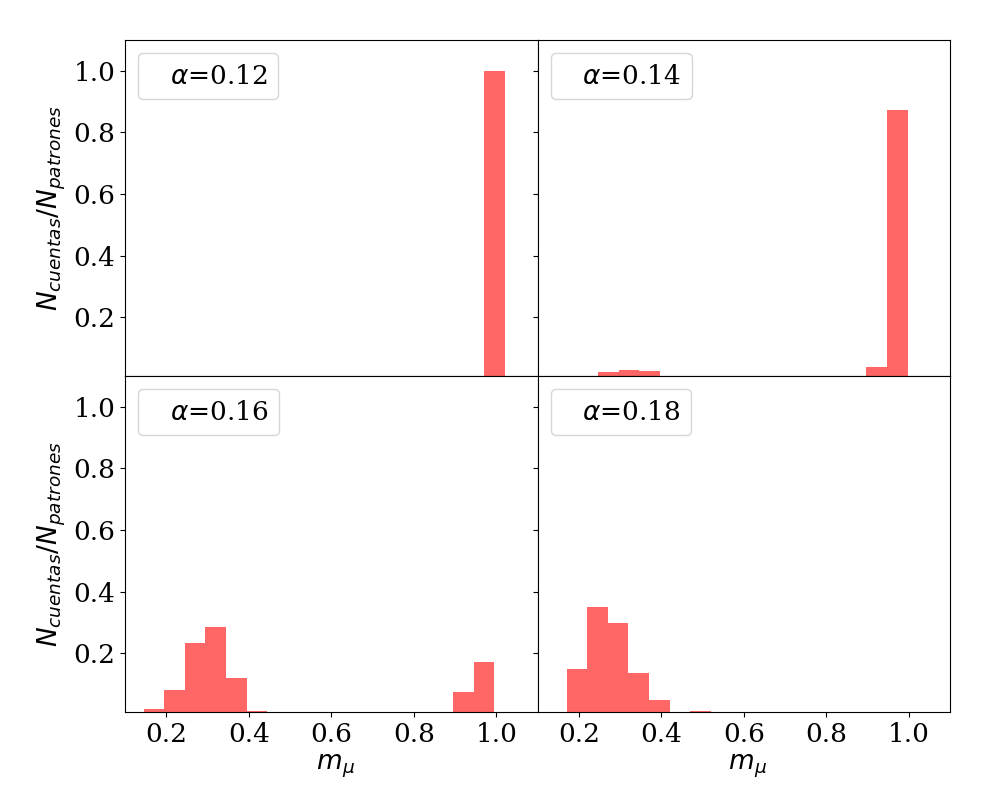
\includegraphics[width=0.5\textwidth]{../Graficos/4000.png}
	\caption{Para $N=4000$}
	\label{fig:4000}
\end{figure}


\section*{Ejercicio II: El modelo de Hopfield con ruido}

\begin{equation}
	s(t+1)=  \begin{cases} 
   +1 & \text{Probabilidad }P(h_i, t, +1) \\
   -1 & \text{Probabilidad }P(h_i, t, -1) 
\end{cases}
\end{equation}

Por lo que el cambio se realiza con una probabilidad

\begin{equation}
	P(h_i, t, \pm 1) = \frac{\exp{(\pm \beta h_i(t))}}{\exp{(- \beta h_i(t))} +\exp{(\beta h_i(t))}}
\end{equation}

Nótese que $P(h_i, t, +1) + P(h_i, t, -1) =1$

\subsubsection{Resultados}

Para $N=4000$, $p=40$, $T=\nicefrac{1}{\beta}$, para $T \in [0.1, 2.0] $

\begin{figure}[H]
	\centering
	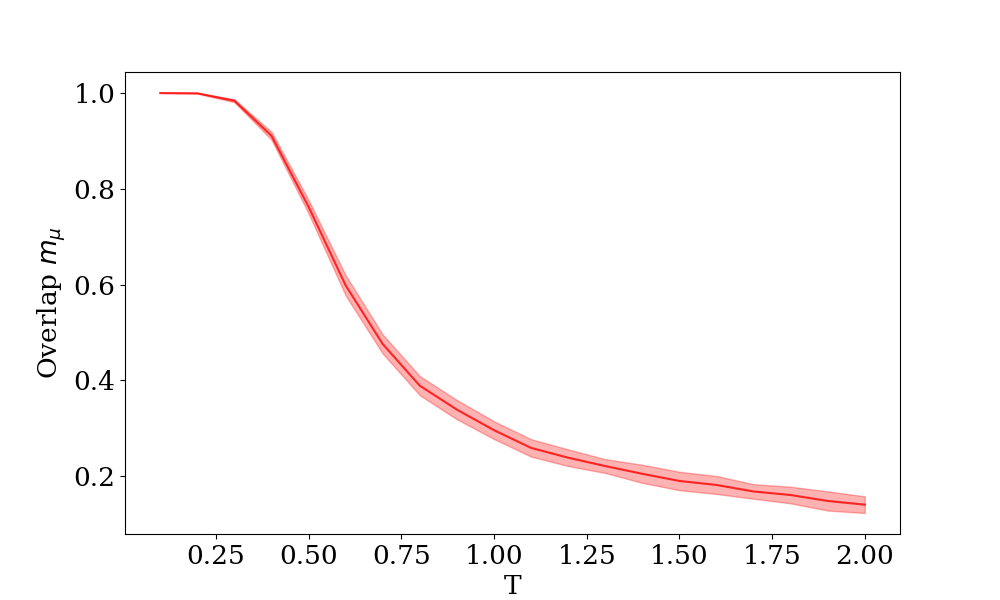
\includegraphics[width=0.5\textwidth]{../Graficos/beta.png}
	\caption{El overlap en función de $T$}
	\label{fig:T}
\end{figure}
donde se ve que para temperaturas bajas, el overlap de la red es cercana a 1, pero a medidad que aumenta el ruido térmico la red empieza a perder la capacidad de memorizar los patrones. 


\end{document}